\subsection{Data Normalization}
\label{sec:DataNormalization}
When comparing multiple entries in a dataset, it might be beneficial to normalize such to obtain a basis for equal comparison.
In the case of numbers being written and detected, such as ours, there might be differences in the colors of the characters when different pens/pencils are used.
This can create unwanted differences between elements in a category, which are else identically, and hence lead to false predictions.
Two normalization algorithms where hence implemented.
These are, min-max normalization and z-score standardization.

Figure \ref{fig:normalization_test_pre-post} shows the result when cross validation is carried out on the data from the 16 people in the class.
In figure \ref{fig:normalization_test_pre-post}, each individual is tested up against the rest of the group without contributing to the training set themselves. 
The two types of normalization are performed both before and after the data reduction using PCA.


\begin{figure}[H]
\centering
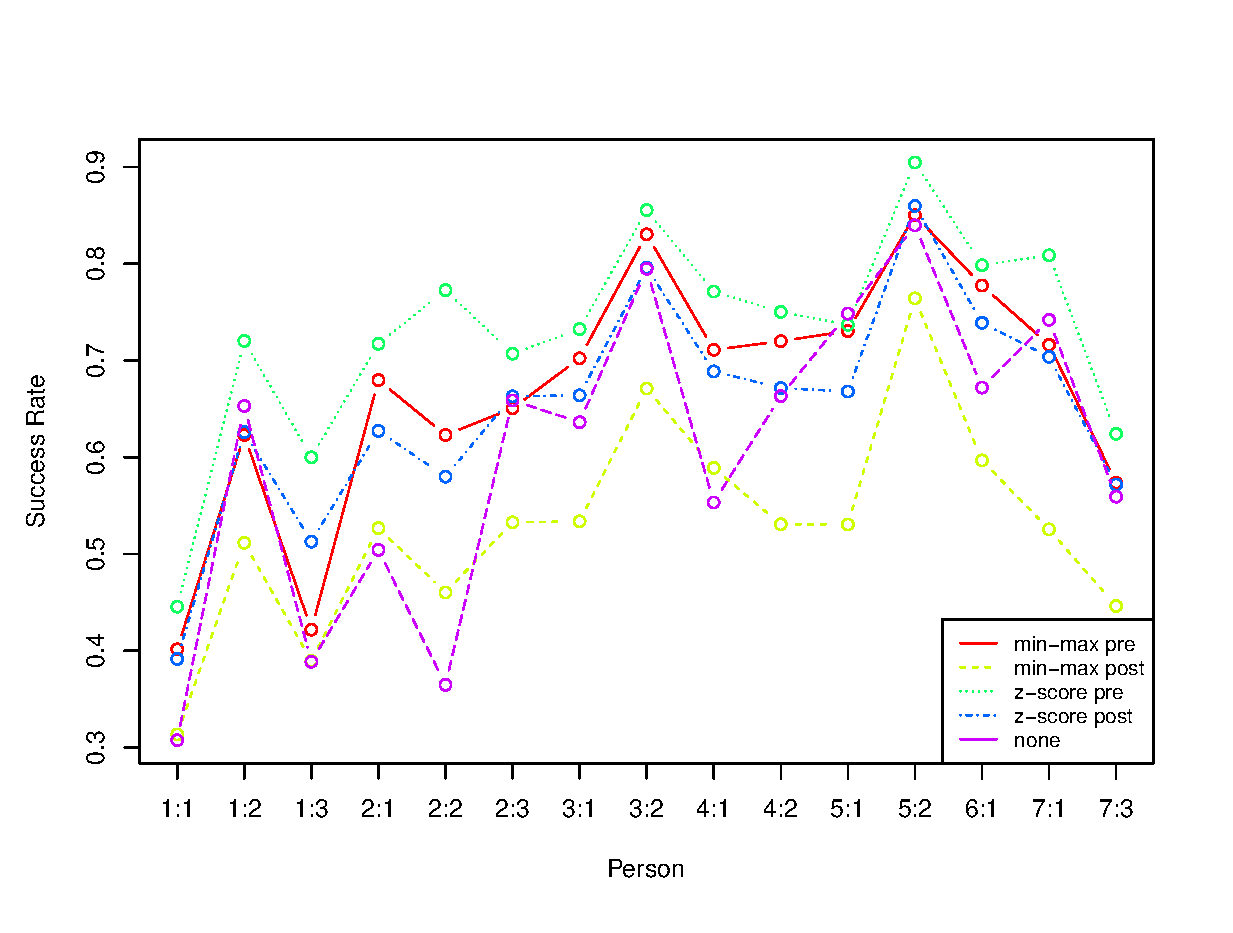
\includegraphics[width = \textwidth]{graphics/graph_normalization}
\caption[Comparison of different students.]{Success rate for detection of characters of on person when not in the training set. 
Data normalized before (pre) and after (post) dataset reduction using PCA.
PCA was set to ensure that 80\% of all variance was included in the data set and K as 10.
The person tested for is given as 'Group':'Member'.
It was tested with 16 people.}
\label{fig:normalization_test_pre-post}
\end{figure}

The mean success rate of figure \ref{fig:normalization_test_pre-post} is listed in table \ref{tab:meanSuccess_normalization_test_pre-post}.
From both the graph and table, it can be concluded that the z-score standardization before the PCA reduction performs, on average, at least 3\% better than the other methods.

The figure \ref{fig:normalization_test_pre-post} also shows that in general all three normalizations, except for the min-max normalization after PCA reduction, is on average, yielding a higher number of correct predictions.

The normalization before the PCA reductions yields a better result in all cases. 
This may be because it enables the PCA to find the features being more responsible for the decision of which category a element belongs to. 
Some of the performance improvement can be because of features of a low variance in their measured value, have a larger relevance as to what the actual category of the elements are.

\begin{table}[H]
\centering
\begin{tabular}{|l|r|}\hline
% 0.5720167 0.4639500 0.6055167 0.5521333 0.5034333
Normalization Method & Mean Success \\ \hline
Min-Max Normalization Pre & 57.2 \% \\ \hline
Min-Max Normalization Post & 46.4 \% \\ \hline
Z-Score Normalization Pre & 60.6 \% \\ \hline
Z-Score Normalization Post & 55.2  \% \\ \hline
No Normalization & 50.3 \% \\ \hline
\end{tabular}
\caption{Mean success rates for normalization test as seen in figure \ref{fig:normalization_test_pre-post}.}
\label{tab:meanSuccess_normalization_test_pre-post}
\end{table}



\subsubsection{Performance Effect when adding a Filter}

\begin{figure}[H]
\centering
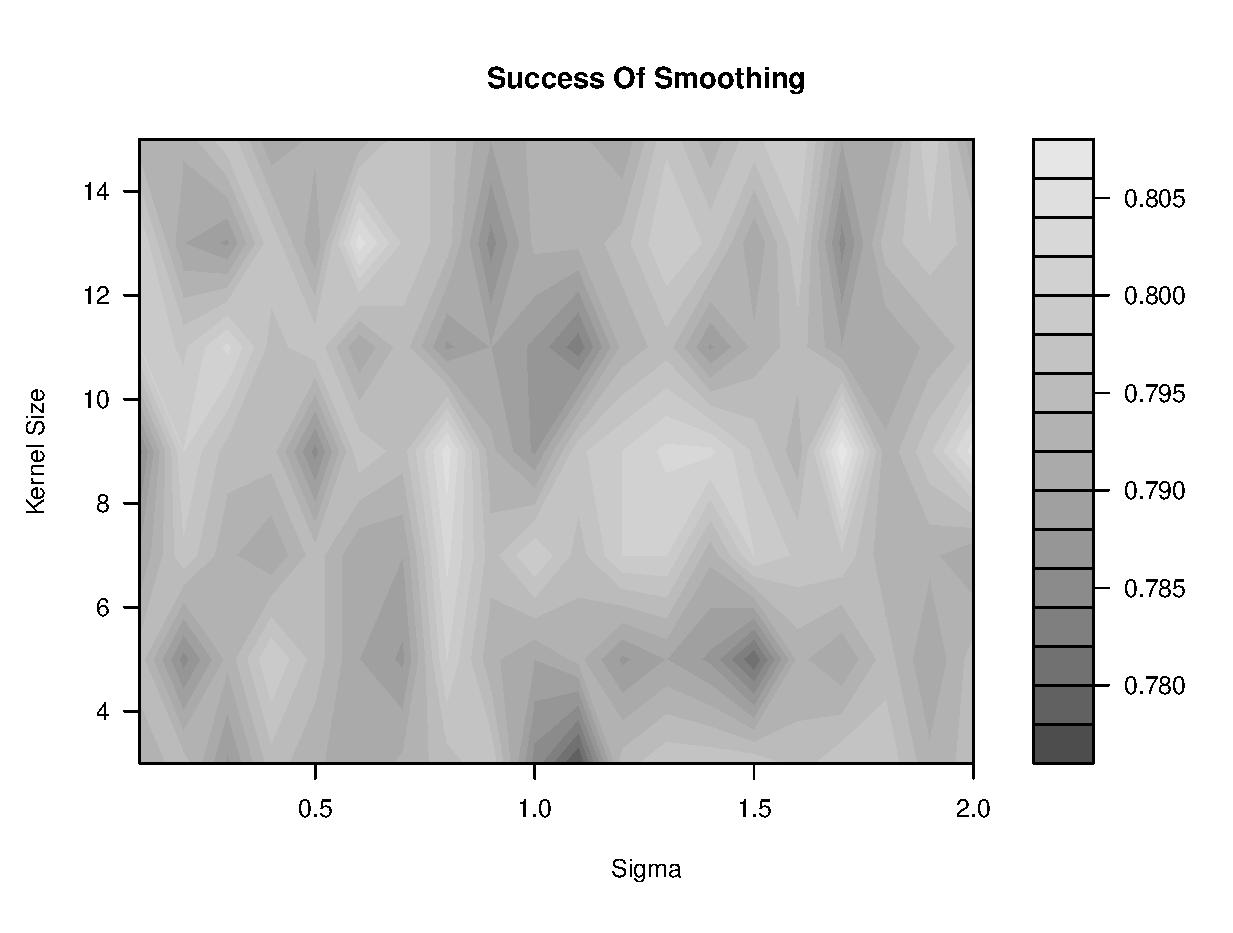
\includegraphics[width = \textwidth]{graphics/success_of_smoothing_contour}
\caption[Optimal smoothing]{Impact of sigma and kernel size when smoothing an image. 
Tested with group 3 member 2's data against 14 other students.
}
\label{fig:smoothing_contour}
\end{figure}

To find the optimal kernel size the success detection rate was plotted with a varying $\sigma$. 
The optimal kernel size is chosen to be 9 pixels wide.
From figure \ref{fig:smoothing_contour} it is concluded that a filter size of 9 is optimal.

Using this knowledge figure \ref{fig:normalization_test_with_smooth} was generated.
The figure compares the unprocessed success rate compared to that of the z-score pre and z-score pre with gaussian smoothing (filter size 9 and sigma 0.7).

 \begin{figure}[H]
 \centering
 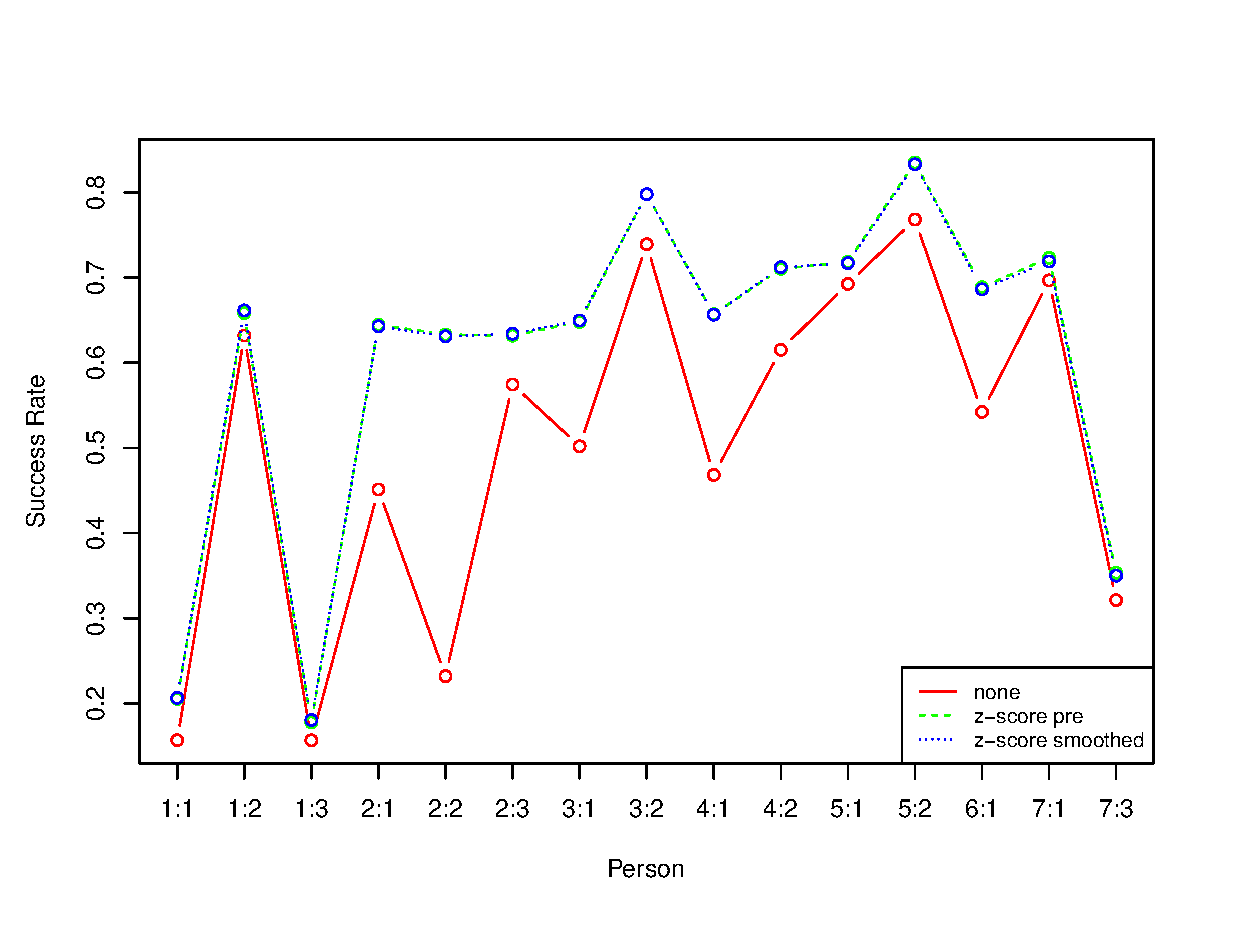
\includegraphics[width = \textwidth]{graphics/graph_normalization_smoothed}
 \caption[Filtered and normalized data.]{Filtered data normalized vs unfiltered normalized data.
 Running each person against the rest of the class in the train set.
 }
 \label{fig:normalization_test_with_smooth}
 \end{figure}

As seen on figure \ref{fig:normalization_test_with_smooth}, then the result of smoothing the data before normalization is not improving the data.
